\documentclass{beamer}
\usepackage[utf8]{inputenc}

\usetheme{Madrid}
\usecolortheme{default}
\usepackage{amsmath,amssymb,amsfonts,amsthm}
\usepackage{txfonts}
\usepackage{tkz-euclide}
\usepackage{listings}
\usepackage{adjustbox}
\usepackage{array}
\usepackage{tabularx}
\usepackage{gvv}
\usepackage{lmodern}
\usepackage{circuitikz}
\usepackage{tikz}
\usepackage{graphicx}
\usepackage{multicol}

\setbeamertemplate{page number in head/foot}[totalframenumber]

\usepackage{tcolorbox}
\tcbuselibrary{minted,breakable,xparse,skins}



\definecolor{bg}{gray}{0.95}
\DeclareTCBListing{mintedbox}{O{}m!O{}}{%
  breakable=true,
  listing engine=minted,
  listing only,
  minted language=#2,
  minted style=default,
  minted options={%
    linenos,
    gobble=0,
    breaklines=true,
    breakafter=,,
    fontsize=\small,
    numbersep=8pt,
    #1},
  boxsep=0pt,
  left skip=0pt,
  right skip=0pt,
  left=25pt,
  right=0pt,
  top=3pt,
  bottom=3pt,
  arc=5pt,
  leftrule=0pt,
  rightrule=0pt,
  bottomrule=2pt,
  toprule=2pt,
  colback=bg,
  colframe=orange!70,
  enhanced,
  overlay={%
    \begin{tcbclipinterior}
    \fill[orange!20!white] (frame.south west) rectangle ([xshift=20pt]frame.north west);
    \end{tcbclipinterior}},
  #3,
}
\lstset{
    language=C,
    basicstyle=\ttfamily\small,
    keywordstyle=\color{blue},
    stringstyle=\color{orange},
    commentstyle=\color{green!60!black},
    numbers=left,
    numberstyle=\tiny\color{gray},
    breaklines=true,
    showstringspaces=false,
}
%------------------------------------------------------------
%This block of code defines the information to appear in the
%Title page
\title %optional
{Signal Processing-1.1.30}
\date\today


\author 
{Josyula G S Avaneesh - EE25BTECH11030}



\begin{document}



\frame{\titlepage}
\begin{frame}{Question}
The frequency spectrum of a signal is shown in the figure. If this signal is ideally
sampled at intervals of 1 ms, then the frequency spectrum of the sampled signal will
be\\
\begin{center}
    \begin{circuitikz}
        % Axes
        \draw [->] (-2,0) -- (2.5,0) node[right] {$\omega$};
        \draw [->] (0,0) -- (0,1.5) node[right] {$|U(j\omega)|$};
        % Triangle Spectrum
        \draw [thick] (-1,0) -- (0,1) -- (1,0);
        % Label
        \node at (1,-0.3) {1 kHz};
    \end{circuitikz}
\end{center}
\begin{enumerate}
    \item[(A)]
    \begin{minipage}[c]{0.8\textwidth}
        \begin{circuitikz}
            \draw [->] (-3,0) -- (3,0) node[right] {$\omega$};
            \draw [->] (0,0) -- (0,1.5) node[right] {$|U(j\omega)|$};
            % Periodic triangles touching at edges
            \draw [thick] (-3,0) -- (-2,1) -- (-1,0) -- (0,1) -- (1,0) -- (2,1) -- (3,0);
        \end{circuitikz}
    \end{minipage}
\end{enumerate}


\end{frame}

\begin{frame}{Question}
\begin{enumerate}
    \item[(B)]
    \begin{minipage}[c]{0.8\textwidth}
        \begin{circuitikz}
            \draw [->] (-3,0) -- (3,0) node[right] {$\omega$};
            \draw [thick] (0,0) -- (0,1.5); % Vertical axis line
            \draw [thick] (-2.8, 1) -- (2.8, 1); % Flat line
        \end{circuitikz}
    \end{minipage}

    \item[(C)]
    \begin{minipage}[c]{0.8\textwidth}
        \begin{circuitikz}
            \draw [->] (-3,0) -- (3,0) node[right] {$\omega$};
            \draw [->] (0,0) -- (0,1.5);
            \draw [thick] (-1,0) -- (0,1) -- (1,0);
        \end{circuitikz}
    \end{minipage}

    \item[(D)]
    \begin{minipage}[c]{0.8\textwidth}
        \begin{circuitikz}
            \draw [->] (-3,0) -- (3.5,0) node[right] {$\omega$};
            \draw [->] (0,0) -- (0,1.5);
            % Overlapping/Aliased "W" shapes
            \draw [thick] (-1.5,0.8) -- (-1,0.4) -- (-0.5,0.8) -- (0,0.4) -- (0.5,0.8) -- (1,0.4) -- (1.5,0.8);
        \end{circuitikz}
    \end{minipage}
\end{enumerate}
\end{frame}

\begin{frame}{Theoretical Solution}

\textbf{Step 1: Analyzing the Message Signal, $m(t)$}
\begin{itemize}
    \item \textbf{The Continuous Signal:} Let the original continuous-time analog signal be the message signal, $m(t)$. 
    \item \textbf{The Frequency Spectrum:} The problem provides the frequency spectrum, $M(\omega)$, which is a triangle spanning symmetrically from $-1 \text{ kHz}$ to $+1 \text{ kHz}$.
    \item \textbf{Maximum Frequency Component ($\omega_M$):} The signal is band-limited with a maximum linear frequency of $f_M = 1 \text{ kHz}$. Converting to angular frequency:
    \[
    \omega_M = 2\pi f_M = 2\pi(1000) \text{ rad/s}
    \]
\end{itemize}
\end{frame}

\begin{frame}{Theoretical Solution} 
\textbf{Step 2: Defining the Sampler and Sampling Frequency ($\omega_s$)}
\begin{itemize}
    \item \textbf{The Impulse Train, $c(t)$:} To sample $m(t)$, it is multiplied by a periodic impulse train $c(t)$ with a sampling period $T_s$.
    \item \textbf{Calculating $\omega_s$:} The given sampling interval is $T_s = 10^{-3} \text{ s}$. The sampling frequency, $\omega_s$, is:
    \[
    \omega_s = \frac{2\pi}{T_s} = 2\pi(1000) \text{ rad/s}
    \]
\end{itemize}
\end{frame}


\begin{frame}{Theoretical Solution} 
\textbf{Step 3: Constructing the Sampled Spectrum}
\begin{itemize}
    \item \textbf{Convolution in Frequency:} Multiplication in the time domain ($s(t) = m(t) \cdot c(t)$) becomes convolution in the frequency domain:
    \[
    S(\omega) = \frac{1}{2\pi} [M(\omega) * C(\omega)]
    \]
    \item \textbf{The Impulse Train in Frequency:} A fundamental property of the Fourier transform is that the transform of a periodic impulse train in time is another infinite impulse train in frequency. So, $C(\omega)$ is represented as:
    \[
    C(\omega) = \frac{2\pi}{T_s} \sum_{n=-\infty}^{\infty} \delta(\omega - n\omega_s)
    \]
    \item \textbf{The Sifting Property:} The Dirac delta function $\delta$ has a ``sifting'' property. When you convolve any spectrum $M(\omega)$ with a shifted impulse $\delta(\omega - \omega_0)$, it simply shifts the entire spectrum to that new center: $M(\omega) * \delta(\omega - \omega_0) = M(\omega - \omega_0)$.
    
\end{itemize}
\end{frame}

\begin{frame}{Theoretical Solution}
\begin{itemize}
\item \textbf{The Infinite Sum:} Substituting $C(\omega)$ into our convolution equation, the $\frac{1}{2\pi}$ and $2\pi$ terms cancel out. We apply the sifting property to every impulse in the infinite train, resulting in an infinite sum of shifted copies of the original spectrum:
    \[
    S(\omega) = \frac{1}{T_s} \sum_{n=-\infty}^{\infty} M(\omega - n\omega_s)
    \]
\end{itemize}
\end{frame}

\begin{frame}{Theoretical Solution}
\begin{itemize}
    \item \textbf{Placing the Replicas:} To visualize this, we evaluate the summation for different integers of $n$:
    \begin{itemize}
        \item \textbf{Baseband ($n=0$):} This term is $M(\omega)$. It is the exact original triangle centered at $0 \text{ rad/s}$, spanning from $-\omega_M$ to $+\omega_M$.
        \item \textbf{First Positive Shift ($n=1$):} This term is $M(\omega - \omega_s)$. It is an identical copy of the triangle, but its center is shifted to $+\omega_s$. It spans from $(\omega_s - \omega_M)$ to $(\omega_s + \omega_M)$.
        \item \textbf{First Negative Shift ($n=-1$):} This term is $M(\omega + \omega_s)$. It is centered at $-\omega_s$ and spans from $(-\omega_s - \omega_M)$ to $(-\omega_s + \omega_M)$.
    \end{itemize}
\end{itemize}
\end{frame}

\begin{frame}{Theoretical Solution}
\textbf{Step 4: Deriving the Nyquist Condition}
\begin{itemize}
    \item \textbf{The Goal (No Overlap):} To accurately recover the original signal, the baseband spectrum ($n=0$) must not mix or overlap with the shifted copies ($n=\pm 1, \pm 2, \dots$).
    \item \textbf{Mathematical Derivation:} 
    \begin{itemize}
        \item The highest frequency of the $n=0$ baseband spectrum is at $+\omega_M$.
        \item The lowest frequency of the adjacent $n=1$ shifted spectrum is at $(\omega_s - \omega_M)$.
        \item To prevent overlap, the start of the next triangle must be strictly greater than or equal to the end of the baseband triangle. Therefore:
        \[
        \omega_s - \omega_M \ge \omega_M
        \]
    \end{itemize}
\end{itemize}
\end{frame}

\begin{frame}{Theoretical Solution}
\begin{itemize}
    \item \textbf{The Nyquist Condition:} Solving the inequality above yields the fundamental rule of sampling:
    \[
    \omega_s \ge 2\omega_M
    \]
    If this condition is not met, the high frequencies fold back into the lower frequencies, causing irreversible distortion known as \textbf{aliasing}.
\end{itemize}
\end{frame}

\begin{frame}{Theoretical Solution}
\textbf{Step 5: Applying to the Problem and Visualizing the Result}
\begin{itemize}
    \item  Here, $\omega_s = \omega_M$. The sampling frequency is exactly half of what it needs to be, guaranteeing severe aliasing.
    \item \textbf{Adding the Overlapping Regions:} Because $\omega_s = \omega_M$, the center of the $n=1$ triangle ($\omega_s$) falls exactly on the right edge of the $n=0$ triangle. The frequency band between $0$ and $\omega_s$:
    \begin{itemize}
        \item In this region, the $n=0$ triangle is a straight line sloping \textit{downward} from its peak to zero.
        \item In the exact same region, the $n=1$ triangle is a straight line sloping \textit{upward} from zero to its peak.
    \end{itemize}
\end{itemize}
\end{frame}

\begin{frame}{Theoretical Solution}
    \textbf{Final Conclusion:} Summing a linearly decreasing function with a linearly increasing function of the exact same slope magnitude yields a constant, flat line. Because the infinite summation $\sum_{n=-\infty}^{\infty}$ continues forever, these overlapping triangles create a continuous, flat horizontal line across the entire spectrum. This perfectly matches option \textbf{(B)}.

    \textbf{Answer: B} 
\end{frame}

\begin{frame}[fragile]
    \frametitle{Python Code}
    \begin{lstlisting}
import numpy as np
import matplotlib.pyplot as plt

# Initialize the frequency axis. 
# The range [-3, 3] kHz is selected to provide a clear view of the baseband and adjacent spectral replicas.
f = np.linspace(-3, 3, 1000)
@np.vectorize  
def original_spectrum(freq):
    if freq < -1 or freq > 1:
        return 0.0
    elif freq >= 0:
        return 1.0 - freq
    else: 
        return 1.0 + freq
# Define the sampling frequency (fs) in kHz.
fs = 1.0
   

\end{lstlisting}
\end{frame}

\begin{frame}[fragile]
    \frametitle{Python Code }
    \begin{lstlisting}
# Initialize an array to store the accumulated sum of all spectral replicas.
sampled_spectrum = np.zeros_like(f)
# Initialize a list to store individual shifted spectra for visualization purposes.
replicas = []
# Simulate the infinite summation of the sampled spectrum.
# A finite range (n = -5 to 5) is utilized as an approximation for computational feasibility.
n_values = range(-5, 6)
for n in n_values:
    # Calculate the frequency shift for the nth harmonic: M(f - n*fs).
    shifted_triangle = original_spectrum(f - n * fs)
    replicas.append(shifted_triangle)
    # Superimpose the shifted spectrum onto the total sampled spectrum array.
    sampled_spectrum += shifted_triangle

\end{lstlisting}
\end{frame}

\begin{frame}[fragile]
    \frametitle{Python Code }
    \begin{lstlisting}
plt.figure(figsize=(10, 6))

# Plot the individual shifted spectral replicas.
for i, replica in enumerate(replicas):
    if i == 5: # Highlights the n=0 baseband spectrum in the legend.
        plt.plot(f, replica, '--', color='blue', alpha=0.6, label='Individual Shifted Spectra')
    else:
        plt.plot(f, replica, '--', color='blue', alpha=0.6)

# Plot the final superimposed spectrum to illustrate aliasing effects.
plt.plot(f, sampled_spectrum, '-', color='red', linewidth=3, label='Final Sampled Spectrum (Sum)')


\end{lstlisting}
\end{frame}

\begin{frame}[fragile]
    \frametitle{Python Code }
    \begin{lstlisting}
# Formatting the plot
plt.title('Frequency Spectrum of Ideally Sampled Signal ($f_s = 1$ kHz)')
plt.xlabel('Frequency (kHz)')
plt.ylabel('Amplitude')
plt.xlim(-3, 3)
plt.ylim(0, 1.5)
plt.grid(True, linestyle=':', alpha=0.7)
plt.legend()

# Displaying the figure
plt.tight_layout()
plt.savefig("../plot.png")
plt.show()
\end{lstlisting}
\end{frame}


\begin{frame}{Plot}
    \centering
    
\includegraphics[width=\columnwidth, height=0.8\textheight, keepaspectratio]{plot.png}     
\end{frame}

\begin{frame}{Theoretical Solution}
{Converting from Frequency Domain to Time Domain}

To find the exact time-domain signal $u(t)$, we must apply the Inverse Fourier Transform to the given frequency spectrum $U(f)$. 

\begin{itemize}
    \item \textbf{Defining the Spectrum:} The given frequency spectrum is a triangle peaking at 1 at $0 \text{ Hz}$, with a maximum frequency $W = 1000 \text{ Hz}$. Mathematically, this is an even piecewise function:
    \[
    U(f) = 
    \begin{cases} 
    1 - \frac{|f|}{W}, & -W \le f \le W \\
    0, & \text{otherwise}
    \end{cases}
    \]

    \item \textbf{Setting up the Integral:} The Inverse Fourier Transform is defined as:
    \[
    u(t) = \int_{-\infty}^{\infty} U(f) e^{j 2\pi ft} \, df
    \]
    Since $U(f) = 0$ outside of $-W$ to $W$, we restrict our integration limits:
    \[
    u(t) = \int_{-W}^{W} \left(1 - \frac{|f|}{W}\right) e^{j 2\pi ft} \, df
    \]
\end{itemize}
    
\end{frame}

\begin{frame}{Theoretical Solution}
{Converting from Frequency Domain to Time Domain}
\begin{itemize}
    \item \textbf{Applying Euler's Formula:} We expand $e^{j 2\pi ft}$ into $\cos(2\pi ft) + j\sin(2\pi ft)$. Because $U(f)$ is an even function (symmetric) and sine is an odd function, the imaginary sine integral evaluates to zero. We are left only with the real cosine part. Because both $U(f)$ and cosine are even, we can integrate from $0$ to $W$ and multiply by 2:
    \[
    u(t) = 2 \int_{0}^{W} \left(1 - \frac{f}{W}\right) \cos(2\pi ft) \, df
    \]
    
    \item \textbf{Splitting the Integral:}
    \[
    u(t) = 2 \underbrace{\int_{0}^{W} \cos(2\pi ft) \, df}_{\text{Part A}} - \frac{2}{W} \underbrace{\int_{0}^{W} f \cos(2\pi ft) \, df}_{\text{Part B}}
    \]

    \item \textbf{Evaluating Part A:}
    \[
    \text{Part A} = \left[ \frac{\sin(2\pi ft)}{2\pi t} \right]_0^W = \frac{\sin(2\pi Wt)}{2\pi t}
    \]

\end{itemize}
    
\end{frame}

\begin{frame}{Theoretical Solution}
{Converting from Frequency Domain to Time Domain}
\begin{itemize}
   \item \textbf{Evaluating Part B (Integration by Parts):} Using $\int u \, dv = uv - \int v \, du$ with $u=f$ and $dv=\cos(2\pi ft)df$:
    \[
    \text{Part B} = \left[ f \frac{\sin(2\pi ft)}{2\pi t} \right]_0^W - \int_{0}^{W} \frac{\sin(2\pi ft)}{2\pi t} \, df
    \]
    \[
    \text{Part B} = W \frac{\sin(2\pi Wt)}{2\pi t} - \left[ -\frac{\cos(2\pi ft)}{(2\pi t)^2} \right]_0^W = W \frac{\sin(2\pi Wt)}{2\pi t} + \frac{\cos(2\pi Wt) - 1}{(2\pi t)^2}
    \]

    \item \textbf{Combining and Simplifying:} Substitute Part A and Part B back into $u(t)$:
    \[
    u(t) = 2 \left[ \frac{\sin(2\pi Wt)}{2\pi t} - \frac{1}{W} \left( W \frac{\sin(2\pi Wt)}{2\pi t} + \frac{\cos(2\pi Wt) - 1}{(2\pi t)^2} \right) \right]
    \]
    Notice how the $\frac{\sin(2\pi Wt)}{2\pi t}$ terms perfectly cancel out:
    \[
    u(t) = -2 \left( \frac{\cos(2\pi Wt) - 1}{W(2\pi t)^2} \right) = 2 \left( \frac{1 - \cos(2\pi Wt)}{W \cdot 4\pi^2 t^2} \right)
    \]
\end{itemize}
    
\end{frame}

\begin{frame}{Theoretical Solution}
{Converting from Frequency Domain to Time Domain}
\begin{itemize}
    \item \textbf{Trigonometric Identity:} Use the half-angle identity $1 - \cos(2\theta) = 2\sin^2(\theta)$, where $\theta = \pi Wt$:
    \[
    u(t) = 2 \left( \frac{2\sin^2(\pi Wt)}{W \cdot 4\pi^2 t^2} \right) = \frac{\sin^2(\pi Wt)}{W \pi^2 t^2}
    \]

    \item \textbf{Final Equation:} To format this into the standard normalized sinc function ($\text{sinc}(x) = \frac{\sin(\pi x)}{\pi x}$), we multiply the numerator and denominator by $W$:
    \[
    u(t) = W \left( \frac{\sin(\pi Wt)}{\pi W t} \right)^2 = W \text{sinc}^2(Wt)
    \]
    Substituting our given $W = 1000$, we arrive at the exact time-domain signal:
    \[
    u(t) = 1000 \text{sinc}^2(1000t)
    \]
\end{itemize}
    
\end{frame}

\begin{frame}{Theoretical Solution}{Sampling the Time Domain signal}
    Now that we have our continuous wave $u(t)$, we sample it by taking discrete snapshots every $1 \text{ ms}$ ($T_s = 0.001 \text{ seconds}$). 

\begin{itemize}
    \item \textbf{Calculating the Samples:} We evaluate $u(t)$ at exactly $t = n(0.001)$, where $n$ is any integer.
    \[
    u[n] = 1000 \text{sinc}^2(1000 \cdot 0.001 \cdot n) = 1000 \text{sinc}^2(n)
    \]
    \item \textbf{The Zero-Crossing Effect:} Because $\text{sinc}(n)$ involves $\sin(\pi n)$, the result is exactly $0$ for every integer \textit{except} zero. At $n=0$, the wave hits its peak amplitude of $1000$.
    \item \textbf{The Result:} Our sampled time-domain signal, $u[n]$, is simply a single, isolated spike (an impulse) of height $1000$ at $t=0$, and $0$ everywhere else.
\end{itemize}

\end{frame}

\begin{frame}{Theoretical Solution}{Frequency Spectrum from the sampled signal}
    To answer the exam question, we convert our newly sampled, single-spike signal $u[n]$ back into the frequency domain using the Discrete-Time Fourier Transform (DTFT).

\begin{itemize}
    \item \textbf{The Impulse Rule:} A fundamental property of the Fourier Transform is that a single discrete impulse in the time domain contains all frequencies in equal, constant amounts.
    \item \textbf{The Result:} The Fourier transform of a single impulse of height $1000$ is simply the constant value $1000$ across all frequencies ($U_s(f) = 1000$). 
    \item \textbf{Conclusion:} This proves that the final sampled frequency spectrum is a continuous, flat horizontal line, making Option (B) the correct answer.
\end{itemize}
\end{frame}

\begin{frame}[fragile]
    \frametitle{Python Code - 2}
    \begin{lstlisting}
import numpy as np
import matplotlib.pyplot as plt

# --- Parameters ---
W = 1000.0          # Bandwidth in Hz
Ts = 0.001          # Sampling interval (1 ms)
t_max = 0.005       # Plot from -5 ms to +5 ms

# --- 1. Continuous Time Signal ---
t_cont = np.linspace(-t_max, t_max, 1000)
u_cont = W * (np.sinc(W * t_cont))**2

# --- 2. Sampled Time Signal ---
t_disc = np.arange(-t_max, t_max + Ts, Ts)
u_disc = W * (np.sinc(W * t_disc))**2

# --- 3. Fourier Transform of the Sampled Signal ---
N = len(u_disc)

\end{lstlisting}
\end{frame}

\begin{frame}[fragile]
    \frametitle{Python Code - 2}
    \begin{lstlisting}
# Calculate the FFT of the discrete samples
# We use ifftshift to correctly align the t=0 point for the algorithm
U_sampled_complex = np.fft.fft(np.fft.ifftshift(u_disc))

# Get the magnitude of the frequency spectrum and center 0 Hz
U_sampled_mag = np.abs(np.fft.fftshift(U_sampled_complex))

# Generate the corresponding frequency axis
freq_axis = np.fft.fftshift(np.fft.fftfreq(N, Ts))

# --- Plotting ---
plt.figure(figsize=(16, 5)) # Made the figure wider to fit 3 plots

\end{lstlisting}
\end{frame}

\begin{frame}[fragile]
    \frametitle{Python Code - 2}
    \begin{lstlisting}
# Subplot 1: Continuous Time Signal
plt.subplot(1, 3, 1)
plt.plot(t_cont * 1000, u_cont, color='blue', linewidth=2)
plt.title('1. Continuous Signal: $u(t)$')
plt.xlabel('Time (ms)')
plt.ylabel('Amplitude')
plt.grid(True, linestyle='--', alpha=0.7)
plt.xlim(-5, 5)

\end{lstlisting}
\end{frame}

\begin{frame}[fragile]
    \frametitle{Python Code - 2}
    \begin{lstlisting}
# Subplot 2: Sampled Time Signal
plt.subplot(1, 3, 2)
plt.plot(t_cont * 1000, u_cont, color='blue', linewidth=1, alpha=0.2)
markerline, stemlines, baseline = plt.stem(t_disc * 1000, u_disc, basefmt="k-")
plt.setp(markerline, color='red', markersize=8)
plt.setp(stemlines, color='red', linewidth=2)
plt.title('2. Sampled Signal: $u(nT_s)$')
plt.xlabel('Time (ms)')
plt.ylabel('Amplitude')
plt.grid(True, linestyle='--', alpha=0.7)
plt.xlim(-5, 5)


\end{lstlisting}
\end{frame}

\begin{frame}[fragile]
    \frametitle{Python Code - 2}
    \begin{lstlisting}
# Subplot 3: Frequency Spectrum of Sampled Signal
plt.subplot(1, 3, 3)
# Plotting the discrete frequency bins connected by a line to show the shape
plt.plot(freq_axis, U_sampled_mag, color='red', linewidth=3, marker='o')
plt.title('3. Spectrum of Sampled Signal: $|U_s(f)|$')
plt.xlabel('Frequency (Hz)')
plt.ylabel('Magnitude')
plt.grid(True, linestyle='--', alpha=0.7)
# Setting Y-axis to clearly show it's a constant, non-zero flat line
plt.ylim(0, max(U_sampled_mag) * 1.5) 

plt.tight_layout()
plt.savefig("../plot2.png")
plt.show()
\end{lstlisting}
\end{frame}

\begin{frame}{Plot}
    \centering
    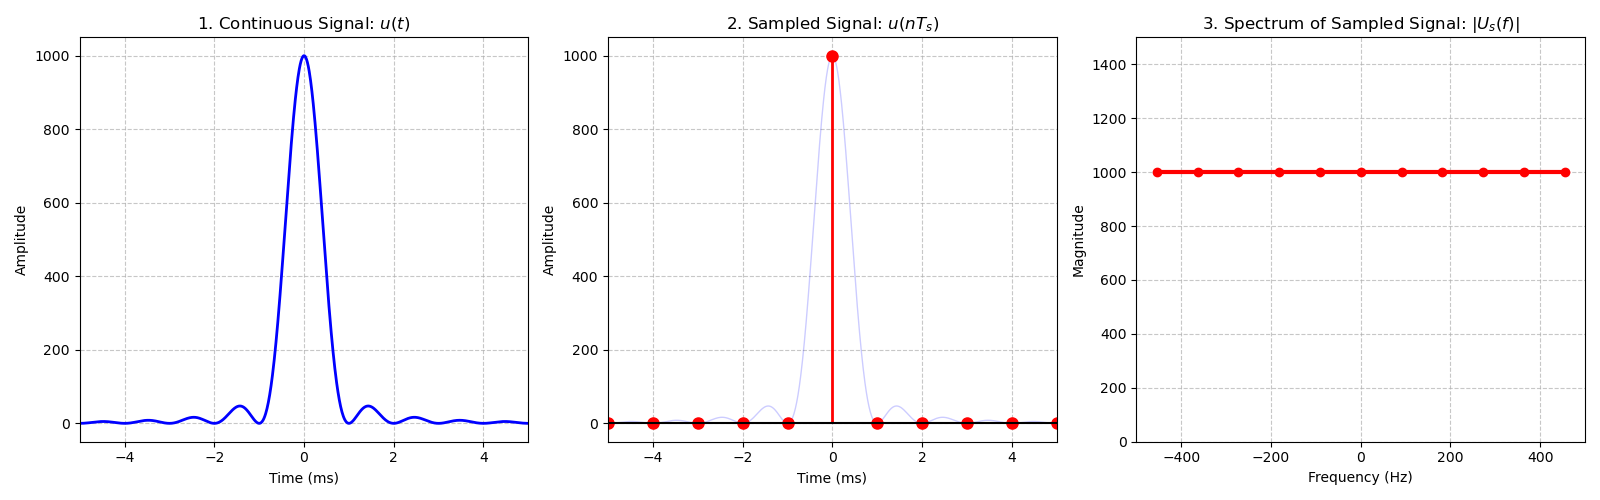
\includegraphics[width=\columnwidth, height=0.8\textheight, keepaspectratio]{plot2.png}     
\end{frame}


\end{document}